\documentclass[10pt,answers]{exam}
\usepackage{mathtools}
\usepackage{amsmath}
\usepackage{amssymb}
\usepackage{xcolor}
\usepackage{graphicx}
\usepackage[top=2.0cm,bottom=2.0cm,left=2.5cm,right=2.5cm]{geometry}
\usepackage{tikz}
\usepackage{float}
\usepackage{multicol}
\usepackage{pgfplots}
\usepackage{lastpage}
\usepackage{siunitx}
\usepackage{xspace}
\usepackage[labelfont=bf]{caption}
\usepackage[hidelinks, urlcolor=blue, linkcolor=blue, colorlinks=true]{hyperref}
\usepackage[capitalize,noabbrev]{cleveref}
\usepackage[absolute]{textpos}
\usepackage{systeme}

\newcommand{\mblue}[1]{\color{blue}\textit{#1}\color{black}}

\newcommand{\R}{\mathbb{R}}
\newcommand{\C}{\mathbb{C}}

\newcommand{\bx}{\mathbf{x}}
\newcommand{\bz}{\mathbf{0}}
\newcommand{\by}{\mathbf{y}}
\newcommand{\bv}{\mathbf{v}}
\newcommand{\be}{\mathbf{e}}
\newcommand{\ba}{\mathbf{a}}
\newcommand{\bb}{\mathbf{b}}
\newcommand{\bc}{\mathbf{c}}
\newcommand{\TT}{ \mathbf{{\tiny T}}}
\newcommand{\T}{ \mathbf{{T}}}

\newcommand{\ds}{\displaystyle}

%% define course title
\newcommand{\course}{MAT185}
\newcommand{\assignmenttitle}{Assignment 3}

%% header and footer
\firstpageheader{}{}{\textbf{{\color{red} Due:} 10:00pm, Tuesday March 18, 2025}}
\firstpageheadrule
\runningheader{}{Page~\thepage~of~\numpages}{\course~--~\assignmenttitle}
\footer{}{}{}

\setlength\parindent{0pt} % no indentation in document

%% formats exam class
\qformat{\textbf{Question \thequestiontitle:}\hfill} % title of question 
\boxedpoints
\pointpoints{mark}{marks}
\pointsinrightmargin
\hpword{Marks:}
\hsword{Your score:}
\unframedsolutions
\totalformat{\boxed{\textnormal{\totalpoints~\if\totalpoints1 mark\else marks\fi}}}
\definecolor{SolutionColor}{rgb}{0,0,1}
\renewcommand{\solutiontitle}{}
\AtBeginEnvironment{solution}{\color{blue}}

% %correct choices in solution
\CorrectChoiceEmphasis{\rm}
\checkedchar{\tikz\draw[blue,fill=blue] (0,0) circle (1ex);}
\newcommand{\emptychoice}{
\begin{tikzpicture}\draw (1,0) circle (1.0ex);\end{tikzpicture}}
\newcommand{\fullchoice}{
\begin{tikzpicture}\draw[blue,fill=blue] (0,0) circle (1ex);\end{tikzpicture}}

% % checkbox which can be used outside the checkbox environment
\newcommand{\TrueChoice}{\ifprintanswers \fullchoice \else \emptychoice \fi}

% % increase distance between checkbox items
\renewcommand{\checkboxeshook}{\setlength{\itemsep}{6pt}}

%% distance between questions and parts
\renewcommand{\questionshook}{\setlength{\parsep}{10pt}}
\renewcommand{\partshook}{\setlength{\parsep}{15pt}}

%% define arrows in text
\newcommand{\arrow}{$\rightarrow$\xspace}
\newcommand{\Arrow}{$\Rightarrow$\xspace}

% % math notation:
%\veccol{1}{2}{3}
\newcommand{\veccol}[3]{
    \begin{bmatrix}
        #1\\
        #2\\
        #3\\
    \end{bmatrix}}
  
%\vecrow{1}{2}{3}
\newcommand{\vecrow}[3]{\left[#1~#2~ #3\right]}

%\matrixTwo{1}{2}{3}{4}
\newcommand{\matrixTwo}[4]{\left[\begin{array}{cc}#1&#2\\#3&#4\end{array}\right]}

% \matrixThree{1}{2}{3}{4}{5}{6}{7}{8}{9}
\newcommand{\matrixThree}[9]{\left[\begin{array}{ccc}#1&#2&#3\\#4&#5&#6\\#7&#8&#9\end{array}\right]}

%\matrixCorner{1}{2}{3}{4}
\newcommand{\matrixCorner}[4]{\left[\begin{array}{ccc}#1& \cdots&#2\\ \vdots & \ddots & \vdots\\#3&
      \cdots&#4\end{array}\right]}

% \nR
\newcommand{\nR}{{}^{n}\mathbb{R}}
% \mR
\newcommand{\mR}{{}^{m}\mathbb{R}}
% \Rn
\newcommand{\Rn}{\mathbb{R}^{n}}
% \nRn
\newcommand{\nRn}{{}^{n}\mathbb{R}^{n}}
% \nRm
\newcommand{\nRm}{{}^{n}\mathbb{R}^{m}}
% \nRm
\newcommand{\mRn}{{}^{m}\mathbb{R}^{n}}
% \mRm
\newcommand{\mRm}{{}^{m}\mathbb{R}^{m}}        

% \u
\renewcommand{\u}{{\bf u}}      
% \v
\renewcommand{\v}{{\bf v}}      
% \w
\newcommand{\w}{{\bf w}}    
% \V
\newcommand{\V}{{\bf V}}                   
       
%% define abbreviations
\newcommand{\row}{\operatorname{row}\,}
\newcommand{\col}{\operatorname{col}\,}
\renewcommand{\dim}{\operatorname{dim}\,}
\renewcommand{\span}{\operatorname{span}\,}
\newcommand{\rank}{\operatorname{rank}\,}
\renewcommand{\ker}{\operatorname{ker}\,}
\newcommand{\nul}{\operatorname{null}\,}
\renewcommand{\det}{\operatorname{det}\,}
\newcommand{\adj}{\operatorname{adj}\,}

\usepackage{xcolor}
\definecolor{dkrgreen}{HTML}{009988} % this is the color-blind friendly teal from below
\definecolor{dkred}{HTML}{EE3377}  % this is the colour-blind friendly magenta from below
\definecolor{blue}{HTML}{1965B0} % this is the colour-blind friendly blue from below
%
% colour-blind-friendly colours from https://personal.sron.nl/~pault/
\definecolor{tolBlue}{HTML}{1965B0}
\definecolor{tolMedBlue}{HTML}{5289C7}
\definecolor{tolLightBlue}{HTML}{7BAFDE} 
\definecolor{tolRed}{HTML}{E8601C} 
\definecolor{tolYellow}{HTML}{F6C141}
\definecolor{tolTeal}{HTML}{009988}
\definecolor{tolCyan}{HTML}{33BBEE}
\definecolor{tolTeal}{HTML}{009988} 
\definecolor{tolOrange}{HTML}{EE7733} 
\definecolor{tolMagenta}{HTML}{EE3377} 
\definecolor{tolGrey}{HTML}{BBBBBB}

%%% This command makes a framed box of a chosen height.
\newcommand{\makenonemptybox}[2]{%
\par\nobreak\vspace{\ht\strutbox}\noindent
\setlength{\fboxrule}{0pt} % set this to 0pt to make invisible
\fbox{%
\parbox[c][#1][t]{\dimexpr\linewidth-2\fboxsep}{
  \hrule width \hsize height 0pt
  \vspace{-0.6cm}
  \color{SolutionColor}#2\color{black}
 }%
}%
\setlength{\fboxrule}{1pt}
}

\newcommand{\makeframednonemptybox}[3]{%
\setlength{\fboxrule}{0.5pt}
\fbox{%
\parbox[c][#1][t]{#2}{%
  \hrule width \hsize height 0pt%
  \vspace{\dimexpr(#1/2-0.1cm)}%
  \color{SolutionColor}#3\color{black}
 }%
}%
\setlength{\fboxrule}{1pt}
}


\begin{document}

\vspace*{-0.5cm}
\begin{center}
  \large
  \textbf{\Large \course~--~Linear Algebra}\\[0.1cm]
  \textbf{\assignmenttitle}
\end{center}
\bigskip

\textbf{\large Instructions:}\\
\normalsize

Please read the {\bf MAT185 Assignment Policies \& FAQ} document for details on
submission policies, collaboration rules and academic integrity, and general
instructions.

\begin{enumerate}


\item \textbf{Submissions are only accepted by}
  \href{https://www.gradescope.ca}{Gradescope}. Do not send anything by email.
  Late submissions are not accepted under any circumstance. Remember you can
  resubmit anytime before the deadline.

\item \textbf{Submit solutions using only this template pdf}.  Your submission
  should be a single pdf with your full written solutions for each question. If
  your solution is not written using this template pdf (scanned print or
  digital) then your submission will not be assessed. Organize your work neatly
  in the space provided.  Do not submit rough work.

\item \textbf{Show your work and justify your steps} on every question but do
  not include extraneous information.  Put your final answer in the box
  provided, if necessary.  We recommend you write draft solutions on separate
  pages and afterwards write your polished solutions here on this template.

\item \textbf{You must fill out and sign the academic integrity statement
    below}; otherwise, you will receive zero for this assignment.

\end{enumerate}

\vspace{10pt}


\textbf{\large Academic Integrity Statement:} \\

%%% Student information


% Student 2
\fbox{
  \begin{minipage}{\textwidth}
    \vspace{0.75cm}
    \makebox[\textwidth]{\large Full Name: Siu, Nelson\enspace\hrulefill}\\[0.75cm]
    \makebox[\textwidth]{\large Student number: 1010940608\enspace\hrulefill}\\
  \end{minipage}
}
\vspace*{0.1in}

% Student 2
\fbox{
  \begin{minipage}{\textwidth}
    \vspace{0.75cm}
    \makebox[\textwidth]{\large Full Name: Cheung, Hei Shing\enspace\hrulefill}\\[0.75cm]
    \makebox[\textwidth]{\large Student number: 1010907823\enspace\hrulefill}\\
  \end{minipage}
}

\bigskip
\large \textbf{I confirm that:}
\normalsize

\begin{itemize} 
\item I have read and followed the policies described in the document {\bf
    MAT185 Assignment Policies \& FAQ}.
\item In particular, I have read and understand the rules for
  collaboration, and permitted resources on assignments as described in
  subsection II of the the aforementioned document. I have not violated
  these rules while completing and writing this assignment.
\item I have not used generative AI in writing this assignment.
\item I understand the consequences of violating the University's academic
  integrity policies as outlined in the
  \href{http://www.governingcouncil.utoronto.ca/policies/behaveac.htm}{Code of
    Behaviour on Academic Matters}. I have not violated them while completing
  and writing this assignment.
\end{itemize}
\bigskip

\large \textbf{By submitting this assignment to Gradescope, I agree that the
  statements above are true.}  \normalsize

\newpage

\begin{questions}
  
   \question 
   
   Consider the real vector space $V = \text{span}\{x^2 e^x, x e^x, e^x\}$.  \textit{No justification needed for parts (a)--(d); just fill in the boxes. :)}

   
    \begin{parts}
     \part Let $T: V \to V$ be the linear transformation corresponding to
     differentiation: $T(v) = v'$.  Using the basis
     $\alpha = \{x^2 e^x, x e^x, e^x\}$ for the domain and the codomain, what
     matrix $[T]_{\alpha \alpha}$ represents this linear transformation?

     %% TO ADD YOUR SOLUTION TO THE RECTANGLE, ADD THE NEXT LINE BEFORE EACH ';'
     %% node[midway,blue]{YOUR ANSWER}
     %%
     %% for example the following has 1, 2, 3 in the three boxes.
     %% \tikz\draw[black] (0,0) rectangle (5ex,5ex) node[midway,blue]{1} ;& \tikz\draw[black] (0,0) rectangle (5ex,5ex) node[midway,blue]{2};&\tikz\draw[black] (0,0) rectangle (5ex,5ex) node[midway,blue]{3}; \\
     %%
     $$[T]_{\alpha \alpha} = \left[\begin{array}{ccc}
                                     \tikz\draw[black] (0,0) rectangle (5ex,5ex) node[midway,blue]{1};& \tikz\draw[black] (0,0) rectangle (5ex,5ex) node[midway,blue]{0};&\tikz\draw[black] (0,0) rectangle (5ex,5ex) node[midway,blue]{0}; \\
                                     \tikz\draw[black] (0,0) rectangle (5ex,5ex) node[midway,blue]{2};& \tikz\draw[black] (0,0) rectangle (5ex,5ex) node[midway,blue]{1};&\tikz\draw[black] (0,0) rectangle (5ex,5ex) node[midway,blue]{0}; \\
                                     \tikz\draw[black] (0,0) rectangle (5ex,5ex) node[midway,blue]{0};& \tikz\draw[black] (0,0) rectangle (5ex,5ex) node[midway,blue]{1};&\tikz\draw[black] (0,0) rectangle (5ex,5ex) node[midway,blue]{1}; \\
          \end{array}\right]$$

        \part Demonstrate that your matrix is correct by computing
        $ [T]_{\alpha \alpha} [v]_\alpha$ for $v =  3 x^2 e^x - 2 x e^x + 6 e^x$ to find 
        $[T(v)]_\alpha =[ 3 x^2 e^x + 4 x e^x + 4 e^x ]_\alpha$.

        %% TO ADD YOUR SOLUTION TO THE RECTANGLE, ADD THE NEXT LINE BEFORE EACH ';'
        %% node[midway,blue]{YOUR ANSWER}
        %% 

        $$[T]_{\alpha \alpha} [v]_\alpha = \left[\begin{array}{ccc}
          \tikz\draw[black] (0,0) rectangle (5ex,5ex) node[midway,blue]{1};& \tikz\draw[black] (0,0) rectangle (5ex,5ex) node[midway,blue]{0};&\tikz\draw[black] (0,0) rectangle (5ex,5ex) node[midway,blue]{0}; \\
          \tikz\draw[black] (0,0) rectangle (5ex,5ex) node[midway,blue]{2};& \tikz\draw[black] (0,0) rectangle (5ex,5ex) node[midway,blue]{1};&\tikz\draw[black] (0,0) rectangle (5ex,5ex) node[midway,blue]{0}; \\
          \tikz\draw[black] (0,0) rectangle (5ex,5ex) node[midway,blue]{0};& \tikz\draw[black] (0,0) rectangle (5ex,5ex) node[midway,blue]{1};&\tikz\draw[black] (0,0) rectangle (5ex,5ex) node[midway,blue]{1}; \\
\end{array}\right]  \left[\begin{array}{c}
\tikz\draw[black] (0,0) rectangle (5ex,5ex) node[midway,blue]{3}; \\
\tikz\draw[black] (0,0) rectangle (5ex,5ex) node[midway,blue]{-2}; \\
\tikz\draw[black] (0,0) rectangle (5ex,5ex) node[midway,blue]{6}; \\
          \end{array}\right] = 
           \left[\begin{array}{c}
\tikz\draw[black] (0,0) rectangle (5ex,5ex) node[midway,blue]{3}; \\
\tikz\draw[black] (0,0) rectangle (5ex,5ex) node[midway,blue]{4}; \\
\tikz\draw[black] (0,0) rectangle (5ex,5ex) node[midway,blue]{4}; \\
          \end{array}\right] = [T(v)]_\alpha$$

        \part What is $[T]_{\alpha \alpha}^{-1}$ for your matrix?  
%        In the
%        language of Calculus, what linear transformation should this matrix
%        represent?

        %% TO ADD YOUR SOLUTION TO THE RECTANGLE, ADD THE NEXT LINE BEFORE EACH ';'
        %% node[midway,blue]{YOUR ANSWER}
        %% 
        $$[T]_{\alpha \alpha}^{-1} = \left[\begin{array}{ccc}
          \tikz\draw[black] (0,0) rectangle (5ex,5ex) node[midway,blue]{1};& \tikz\draw[black] (0,0) rectangle (5ex,5ex) node[midway,blue]{0};&\tikz\draw[black] (0,0) rectangle (5ex,5ex) node[midway,blue]{0}; \\
          \tikz\draw[black] (0,0) rectangle (5ex,5ex) node[midway,blue]{-2};& \tikz\draw[black] (0,0) rectangle (5ex,5ex) node[midway,blue]{1};&\tikz\draw[black] (0,0) rectangle (5ex,5ex) node[midway,blue]{0}; \\
          \tikz\draw[black] (0,0) rectangle (5ex,5ex) node[midway,blue]{2};& \tikz\draw[black] (0,0) rectangle (5ex,5ex) node[midway,blue]{-1};&\tikz\draw[black] (0,0) rectangle (5ex,5ex) node[midway,blue]{1}; \\
         \end{array}\right]$$

        %Do not change the height of this box. Your work must fit inside it.
        \makenonemptybox{1.0cm}{
          %Add your explanations here!      
          
          %end of your answer    
        }
        \vspace{-1cm}

        \part Using your $[T]_{\alpha \alpha}^{-1}$, find $v \in V$ such that $v'(x) = x^2 e^x$.    

        %% TO ADD YOUR SOLUTION TO THE RECTANGLE, ADD THE NEXT LINE BEFORE EACH ';'
        %% node[midway,blue]{YOUR ANSWER}
        %% 
        $$[T]_{\alpha \alpha}^{-1} [v]_\alpha = \left[\begin{array}{ccc}
           \tikz\draw[black] (0,0) rectangle (5ex,5ex) node[midway,blue]{1};& \tikz\draw[black] (0,0) rectangle (5ex,5ex) node[midway,blue]{0};&\tikz\draw[black] (0,0) rectangle (5ex,5ex) node[midway,blue]{0}; \\
           \tikz\draw[black] (0,0) rectangle (5ex,5ex) node[midway,blue]{-2};& \tikz\draw[black] (0,0) rectangle (5ex,5ex) node[midway,blue]{1};&\tikz\draw[black] (0,0) rectangle (5ex,5ex) node[midway,blue]{0}; \\
           \tikz\draw[black] (0,0) rectangle (5ex,5ex) node[midway,blue]{2};& \tikz\draw[black] (0,0) rectangle (5ex,5ex) node[midway,blue]{-1};&\tikz\draw[black] (0,0) rectangle (5ex,5ex) node[midway,blue]{1}; \\
          \end{array}\right]  \left[\begin{array}{c}
\tikz\draw[black] (0,0) rectangle (5ex,5ex) node[midway,blue]{1}; \\
\tikz\draw[black] (0,0) rectangle (5ex,5ex) node[midway,blue]{0}; \\
\tikz\draw[black] (0,0) rectangle (5ex,5ex) node[midway,blue]{0}; \\
          \end{array}\right] = 
           \left[\begin{array}{c}
\tikz\draw[black] (0,0) rectangle (5ex,5ex) node[midway,blue]{1}; \\
\tikz\draw[black] (0,0) rectangle (5ex,5ex) node[midway,blue]{-2}; \\
\tikz\draw[black] (0,0) rectangle (5ex,5ex) node[midway,blue]{2}; \\
          \end{array}\right] = [T^{-1}(v)]_\alpha$$
       $v(x)$= \makeframednonemptybox{1cm}{6cm}{$x^2e^x - 2xe^x + 2e^x$}
        
    \part You've learnt that a function has infinitely many antiderivatives.
    Why is it that this method has found only one of them?

    %%% Do not change the height of this box. Your work must fit inside it.
    \makenonemptybox{2.5cm}{
      %%% Add your explanations here!      
      In general, we have:
      $$\int f(x) dx = F(x) + c$$ 
      ,where $F(x)$ is the antiderivative of $f(x)$. \\
      The linear transformation $T$ maps to the special case $c=0$. The constant function is not spanned by the bases of vector space $V$, so the antiderivative found is unique with $c=0$. In general, linear transformation that represent the antiderivative cannot have non-zero constant such that the additivity property of the linear transformation is preserved. (i. e. $T(f+g) = F + G + c = T(f) + T(g) = F + G + 2c$)
      %%% end of your answer    
    } 

    
  \end{parts}
  
  
  \question  
  
  \begin{parts}
    \part What is a parametrized curve that represents the line segment that
    connects $(x_0,y_0)$ to $(x_1,y_1)$?  That is, what is an $\ell(t)$ such
    that $\ell(0) = (x_0,y_0)$, $\ell(1) = (x_1,y_1)$, and
    $\{ \ell(t) \mid 0 \leq t \leq 1 \}$ is a line segment?

    %%% Do not change the height of this box. Your work must fit inside it.
    \makenonemptybox{2cm}{
      %%% Add your explanations here!      
      $$\ell(t) = (x(t), y(t)) = (1-t)(x_0, y_0) + t(x_1, y_1),\, 0 \leq t \leq 1$$
      Putting into standard form, we have:
      $$\ell(t) = (x_0, y_0) + t(x_1 - x_0, y_1 - y_0)$$
    } 
   
    \part Consider the linear transformation $T: \R^2 \to \R^2$ where
    $T((x,y)) = (2x+3y,-6x+y)$.  What is the image of the above line segment
    $\{ \ell(t) \mid 0 \leq t \leq 1 \}$ under this linear transformation?

    %%% Do not change the height of this box. Your work must fit inside it.
    \makenonemptybox{3cm}{
      %%% Add your explanations here!      
      For $0 \leq t \leq 1$, we have:
      $$T(\ell(t)) = (2x(t) + 3y(t), -6x(t) + y(t)) = (2(1-t)x_0 + 2tx_1 + 3(1-t)y_0 + 3ty_1, -6(1-t)x_0 - 6tx_1 + (1-t)y_0 + ty_1)$$
      Simplifying, we have the line segment connecting $(2x_0 + 3y_0, -6x_0 + y_0)$ to $(2x_1 + 3y_1, -6x_1 + y_1)$:
      $$T(\ell(t)) = ((1-t)(2x_0 + 3y_0) + t(2x_1 + 3y_1), (1-t)(-6x_0 + y_0) + t(-6x_1 + y_1))$$
      Putting into standard form, we have:
      $$T(\ell(t)) = (2x_0 + 3y_0, -6x_0 + y_0) + t(2(x_1 - x_0) + 3(y_1 - y_0), -6(x_1 - x_0) + (y_1 - y_0))$$
      %%% end of your answer    
    }
          
    \part Consider a general linear transformation $T: \R^2 \to \R^2$;  that is, $T((x,y)) = (a_{11} x + a_{12} y, a_{21} x + a_{22} y )$ where $a_{11}, a_{12}, a_{21}, a_{22} \in \R$.  Let 
 $\ell \subseteq \R^2$ be a line in the plane.  In ten words or less, what is the image of $\ell$?  That is, what is $T(\ell)$?

    %%% Do not change the height of this box. Your work must fit inside it.
    \makenonemptybox{1cm}{
      %%% Add your explanations here!      
      $T(\ell)$ is a line or a point in $\R^2$.
      %%% end of your answer    
    }
    \vspace{-1cm}
       
   \part  \textit{No justification is needed. You can select more than one answer.} Let $P \subseteq \R^2$ be a polygon\footnote{Here are the \href{https://www.geeksforgeeks.org/polygon/}{\underline{types of polygons}} we mean here.  Think about both regular and irregular ones, please.} and consider a general linear transformation as in part (c).  The image of $P$ under
   $T$ could be
   
   \vspace{-.5cm}
   
    \begin{checkboxes}
      \choice a circle
      \correctchoice a point
      \correctchoice a line segment
      \correctchoice a polygon
      \choice something else
      %REPLACE \choice with \correctchoice TO MARK YOUR ANSWER 
    \end{checkboxes}
   
  \end{parts}
   
  \newpage
  
  \question  
   
  In the following, you will consider a sequence of linear transformations.  For
  each linear transformation you will asked to draw the image of a square under
  the linear transformation.
    \textit{No justification needed for parts (a)--(f); just fill in the boxes. :)}

  \begin{parts} 
  
  \part Consider the linear transformation $T: \R^2 \to \R^2$ given by
  $T((x,y)) = (x,x/2+y)$.  In the domain, draw the unit square
  $\mathcal{S} = \{ (x,y) \mid 0 \leq x \leq 1, 0 \leq y \leq 1 \}$.  In the
  codomain draw the image of the unit square $T(\mathcal{S})$.
  
  \begin{center}
  
    \begin{minipage}{.15\textwidth}
      \begin{center}
        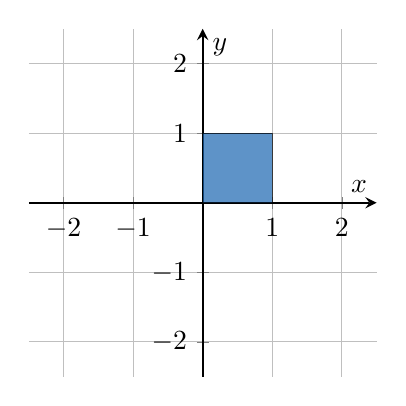
\begin{tikzpicture}
          \begin{axis}[axis x line=center,axis line style = thick,axis y
            line=center,axis
            equal,xmin=-2.5,ymin=-2.5,xmax=2.5,ymax=2.5,xtick={-2,-1,...,2},ytick={-2,-1,...,2},grid=both,xlabel={$x$},ylabel={$y$},width=6cm,height=6cm]
            \addplot[fill=blue,opacity=0.7] coordinates {(0,0) (1,0) (1,1) (0,1)};
          \end{axis}
        \end{tikzpicture}
      \end{center}
    \end{minipage}
    \hspace{2cm}
    \begin{minipage}{.3\textwidth}
      \begin{tikz}
        \draw[-latex,line width=2pt] (1,0) to[out=25,in=155] node[above]{$T$} (2,0);
      \end{tikz}

      \vspace{2cm}
    \end{minipage}
    \hspace{-4.5cm}
    \begin{minipage}{.35\textwidth}
      \begin{center}
        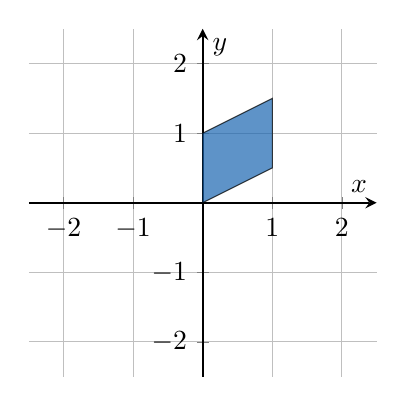
\begin{tikzpicture}
          \begin{axis}[axis x line=center,axis line style = thick,axis y
            line=center,axis
            equal,xmin=-2.5,ymin=-2.5,xmax=2.5,ymax=2.5,xtick={-2,-1,...,2},ytick={-2,-1,...,2},grid=both,xlabel={$x$},ylabel={$y$},width=6cm,height=6cm]
            \addplot[fill=blue,opacity=0.7] coordinates {(0,0) (1,0.5) (1,1.5) (0,1)};
          \end{axis}
        \end{tikzpicture}
      \end{center}
    \end{minipage}
  \end{center}
  What is the area of $\mathcal{S}$?  What is the area of its image
  $T(\mathcal{S})$?  If $\alpha$ is the standard basis for $\R^2$, what is the
  matrix $[T]_{\alpha \alpha}$ that represents the linear transformation $T$?
  What is $\mbox{det} [T]_{\alpha \alpha}$?

  \begin{minipage}{.2\textwidth}
    Area of $\mathcal{S}=$ \makeframednonemptybox{0.5cm}{0.5cm}{1
    }
  \end{minipage}
  \hspace{.2cm}
  \begin{minipage}{.25\textwidth}
    Area of $T(\mathcal{S})=$ \makeframednonemptybox{0.5cm}{0.5cm}{1
    }
  \end{minipage}
  \hspace{.2cm}
  \begin{minipage}{.25\textwidth}
    %% TO ADD YOUR SOLUTION TO THE RECTANGLE, ADD THE NEXT LINE BEFORE EACH ';'
    %% node[midway,blue]{YOUR ANSWER}
    %% 
  $[T]_{\alpha \alpha} = \left[\begin{array}{cc}
            \tikz\draw[black] (0,0) rectangle (5ex,5ex) node[midway,blue]{1};& \tikz\draw[black] (0,0) rectangle (5ex,5ex) node[midway,blue]{0}; \\
            \tikz\draw[black] (0,0) rectangle (5ex,5ex) node[midway,blue]{$\frac{1}{2}$};& \tikz\draw[black] (0,0) rectangle (5ex,5ex) node[midway,blue]{1}; \\
          \end{array}\right]$
   \end{minipage}
   \hspace{.8cm}
   \begin{minipage}{.2\textwidth}
     $\mbox{det} [T]_{\alpha \alpha}=$\makeframednonemptybox{0.5cm}{0.5cm}{1
    }
   \end{minipage}
   
   \part Consider the linear transformation $T: \R^2 \to \R^2$ given by
   $T((x,y)) = (2x,2y)$.  In the domain, draw the unit square
   $\mathcal{S} = \{ (x,y) \mid 0 \leq x \leq 1, 0 \leq y \leq 1 \}$.  In the
   codomain draw the image of the unit square $T(\mathcal{S})$.
   
   \begin{center}
     
     \begin{minipage}{.15\textwidth}
       \begin{center}
         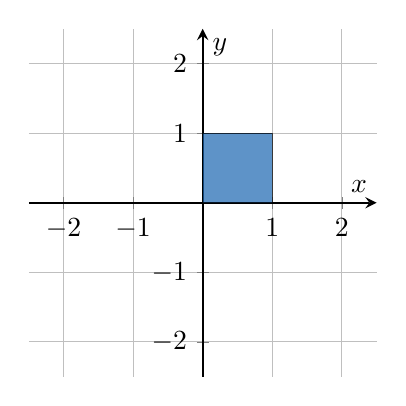
\begin{tikzpicture}
           \begin{axis}[axis x line=center,axis line style = thick,axis y
             line=center,axis
             equal,xmin=-2.5,ymin=-2.5,xmax=2.5,ymax=2.5,xtick={-2,-1,...,2},ytick={-2,-1,...,2},grid=both,xlabel={$x$},ylabel={$y$},width=6cm,height=6cm]
            \addplot[fill=blue,opacity=0.7] coordinates {(0,0) (1,0) (1,1) (0,1)};
           \end{axis}
         \end{tikzpicture}
       \end{center}
     \end{minipage}
     \hspace{2cm}
     \begin{minipage}{.3\textwidth}
       \begin{tikz}
         \draw[-latex,line width=2pt] (1,0) to[out=25,in=155] node[above]{$T$} (2,0);
       \end{tikz}

       \vspace{2cm}
     \end{minipage}
     \hspace{-4.5cm}
     \begin{minipage}{.35\textwidth}
       \begin{center}
         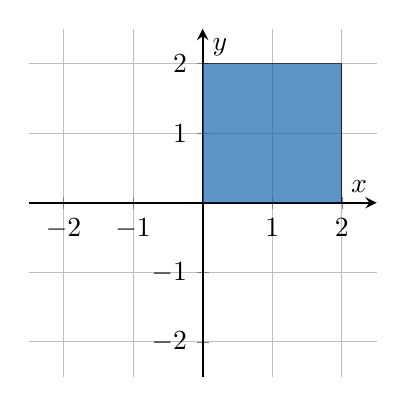
\begin{tikzpicture}
           \begin{axis}[axis x line=center,axis line style = thick,axis y
             line=center,axis
             equal,xmin=-2.5,ymin=-2.5,xmax=2.5,ymax=2.5,xtick={-2,-1,...,2},ytick={-2,-1,...,2},grid=both,xlabel={$x$},ylabel={$y$},width=6cm,height=6cm]
            \addplot[fill=blue,opacity=0.7] coordinates {(0,0) (2,0) (2,2) (0,2)};
           \end{axis}
         \end{tikzpicture}
       \end{center}
     \end{minipage}
   \end{center}
   What is the area of $\mathcal{S}$?  What is the area of its image
   $T(\mathcal{S})$?  If $\alpha$ is the standard basis for $\R^2$, what is the
   matrix $[T]_{\alpha \alpha}$ that represents the linear transformation $T$?
   What is $\mbox{det} [T]_{\alpha \alpha}$?
   
\begin{minipage}{.2\textwidth}
    Area of $\mathcal{S}=$ \makeframednonemptybox{0.5cm}{0.5cm}{1
    }
  \end{minipage}
  \hspace{.2cm}
  \begin{minipage}{.25\textwidth}
    Area of $T(\mathcal{S})=$ \makeframednonemptybox{0.5cm}{0.5cm}{4
    }
  \end{minipage}
  \hspace{.2cm}
  \begin{minipage}{.25\textwidth}
    %% TO ADD YOUR SOLUTION TO THE RECTANGLE, ADD THE NEXT LINE BEFORE EACH ';'
    %% node[midway,blue]{YOUR ANSWER}
    %% 
  $[T]_{\alpha \alpha} = \left[\begin{array}{cc}
            \tikz\draw[black] (0,0) rectangle (5ex,5ex) node[midway,blue]{2};& \tikz\draw[black] (0,0) rectangle (5ex,5ex) node[midway,blue]{0}; \\
            \tikz\draw[black] (0,0) rectangle (5ex,5ex) node[midway,blue]{0};& \tikz\draw[black] (0,0) rectangle (5ex,5ex) node[midway,blue]{2}; \\
          \end{array}\right]$
   \end{minipage}
   \hspace{.8cm}
   \begin{minipage}{.2\textwidth}
     $\mbox{det} [T]_{\alpha \alpha}=$\makeframednonemptybox{0.5cm}{0.5cm}{4
    }
   \end{minipage}
   
   \newpage
   
   
   \part Consider the linear transformation $T: \R^2 \to \R^2$ given by
   $T((x,y)) = (2x,y/2)$.  In the domain, draw the unit square
   $\mathcal{S} = \{ (x,y) \mid 0 \leq x \leq 1, 0 \leq y \leq 1 \}$.  In the
   codomain draw the image of the unit square $T(\mathcal{S})$.
   
   \begin{center}
     
     \begin{minipage}{.15\textwidth}
       \begin{center}
         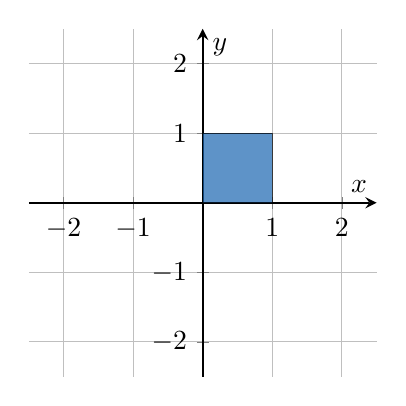
\begin{tikzpicture}
           \begin{axis}[axis x line=center,axis line style = thick,axis y
             line=center,axis
             equal,xmin=-2.5,ymin=-2.5,xmax=2.5,ymax=2.5,xtick={-2,-1,...,2},ytick={-2,-1,...,2},grid=both,xlabel={$x$},ylabel={$y$},width=6cm,height=6cm]
            \addplot[fill=blue,opacity=0.7] coordinates {(0,0) (1,0) (1,1) (0,1)};
           \end{axis}
         \end{tikzpicture}
       \end{center}
     \end{minipage}
     \hspace{2cm}
     \begin{minipage}{.3\textwidth}
       \begin{tikz}
         \draw[-latex,line width=2pt] (1,0) to[out=25,in=155] node[above]{$T$} (2,0);
       \end{tikz}
       
       \vspace{2cm}
     \end{minipage}
     \hspace{-4.5cm}
     \begin{minipage}{.35\textwidth}
       \begin{center}
         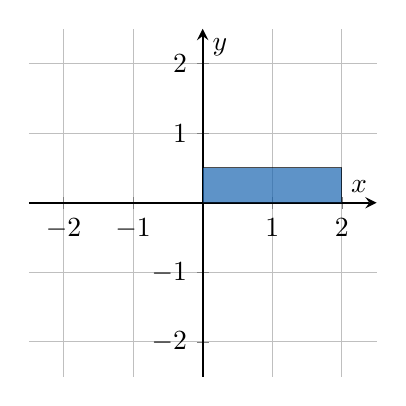
\begin{tikzpicture}
           \begin{axis}[axis x line=center,axis line style = thick,axis y
             line=center,axis
             equal,xmin=-2.5,ymin=-2.5,xmax=2.5,ymax=2.5,xtick={-2,-1,...,2},ytick={-2,-1,...,2},grid=both,xlabel={$x$},ylabel={$y$},width=6cm,height=6cm]
            \addplot[fill=blue,opacity=0.7] coordinates {(0,0) (2,0) (2,0.5) (0,0.5)};
           \end{axis}
         \end{tikzpicture}
       \end{center}
     \end{minipage}
   \end{center}
   What is the area of $\mathcal{S}$?  What is the area of its image
   $T(\mathcal{S})$?  If $\alpha$ is the standard basis for $\R^2$, what is the
   matrix $[T]_{\alpha \alpha}$ that represents the linear transformation $T$?
   What is $\mbox{det} [T]_{\alpha \alpha}$?
   
\begin{minipage}{.2\textwidth}
    Area of $\mathcal{S}=$ \makeframednonemptybox{0.5cm}{0.5cm}{1
    }
  \end{minipage}
  \hspace{.2cm}
  \begin{minipage}{.25\textwidth}
    Area of $T(\mathcal{S})=$ \makeframednonemptybox{0.5cm}{0.5cm}{1
    }
  \end{minipage}
  \hspace{.2cm}
  \begin{minipage}{.25\textwidth}
    %% TO ADD YOUR SOLUTION TO THE RECTANGLE, ADD THE NEXT LINE BEFORE EACH ';'
    %% node[midway,blue]{YOUR ANSWER}
    %% 
  $[T]_{\alpha \alpha} = \left[\begin{array}{cc}
            \tikz\draw[black] (0,0) rectangle (5ex,5ex) node[midway,blue]{2};& \tikz\draw[black] (0,0) rectangle (5ex,5ex) node[midway,blue]{0}; \\
            \tikz\draw[black] (0,0) rectangle (5ex,5ex) node[midway,blue]{0};& \tikz\draw[black] (0,0) rectangle (5ex,5ex) node[midway,blue]{$\frac{1}{2}$}; \\
          \end{array}\right]$
   \end{minipage}
   \hspace{.8cm}
   \begin{minipage}{.2\textwidth}
     $\mbox{det} [T]_{\alpha \alpha}=$\makeframednonemptybox{0.5cm}{0.5cm}{1
    }
   \end{minipage}

      \part Consider the linear transformation $T: \R^2 \to \R^2$ given by
      $T((x,y)) = (-y,x)$.  In the domain, draw the unit square
      $\mathcal{S} = \{ (x,y) \mid 0 \leq x \leq 1, 0 \leq y \leq 1 \}$.  In the
      codomain draw the image of the unit square $T(\mathcal{S})$.
      
      \begin{center}
        
        \begin{minipage}{.15\textwidth}
          \begin{center}
            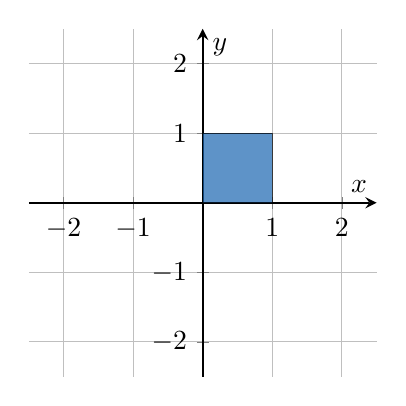
\begin{tikzpicture}
              \begin{axis}[axis x line=center,axis line style = thick,axis y
                line=center,axis
                equal,xmin=-2.5,ymin=-2.5,xmax=2.5,ymax=2.5,xtick={-2,-1,...,2},ytick={-2,-1,...,2},grid=both,xlabel={$x$},ylabel={$y$},width=6cm,height=6cm]
              \addplot[fill=blue,opacity=0.7] coordinates {(0,0) (1,0) (1,1) (0,1)};
              \end{axis}
            \end{tikzpicture}
          \end{center}
        \end{minipage}
        \hspace{2cm}
        \begin{minipage}{.3\textwidth}
          \begin{tikz}
            \draw[-latex,line width=2pt] (1,0) to[out=25,in=155] node[above]{$T$} (2,0);
          \end{tikz}
          
          \vspace{2cm}
        \end{minipage}
        \hspace{-4.5cm}
        \begin{minipage}{.35\textwidth}
          \begin{center}
            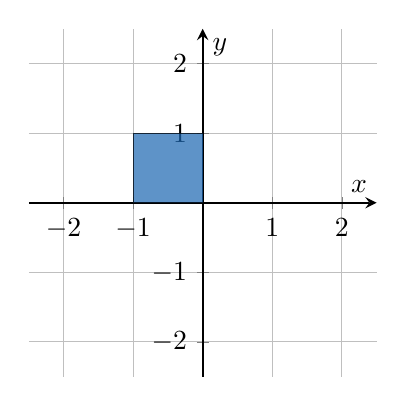
\begin{tikzpicture}
              \begin{axis}[axis x line=center,axis line style = thick,axis y
                line=center,axis
                equal,xmin=-2.5,ymin=-2.5,xmax=2.5,ymax=2.5,xtick={-2,-1,...,2},ytick={-2,-1,...,2},grid=both,xlabel={$x$},ylabel={$y$},width=6cm,height=6cm]
                \addplot[fill=blue,opacity=0.7] coordinates {(0,0) (-1,0) (-1,1) (0,1)};
              \end{axis}
            \end{tikzpicture}
          \end{center}
        \end{minipage}
      \end{center}
      What is the area of $\mathcal{S}$?  What is the area of its image
      $T(\mathcal{S})$?  If $\alpha$ is the standard basis for $\R^2$, what is
      the matrix $[T]_{\alpha \alpha}$ that represents the linear transformation
      $T$?  What is $\mbox{det} [T]_{\alpha \alpha}$?
      
\begin{minipage}{.2\textwidth}
    Area of $\mathcal{S}=$ \makeframednonemptybox{0.5cm}{0.5cm}{1
    }
  \end{minipage}
  \hspace{.2cm}
  \begin{minipage}{.25\textwidth}
    Area of $T(\mathcal{S})=$ \makeframednonemptybox{0.5cm}{0.5cm}{1
    }
  \end{minipage}
  \hspace{.2cm}
  \begin{minipage}{.25\textwidth}
    %% TO ADD YOUR SOLUTION TO THE RECTANGLE, ADD THE NEXT LINE BEFORE EACH ';'
    %% node[midway,blue]{YOUR ANSWER}
    %% 
  $[T]_{\alpha \alpha} = \left[\begin{array}{cc}
            \tikz\draw[black] (0,0) rectangle (5ex,5ex) node[midway,blue]{0};& \tikz\draw[black] (0,0) rectangle (5ex,5ex) node[midway,blue]{-1}; \\
            \tikz\draw[black] (0,0) rectangle (5ex,5ex) node[midway,blue]{1};& \tikz\draw[black] (0,0) rectangle (5ex,5ex) node[midway,blue]{0}; \\
          \end{array}\right]$
   \end{minipage}
   \hspace{.8cm}
   \begin{minipage}{.2\textwidth}
     $\mbox{det} [T]_{\alpha \alpha}=$\makeframednonemptybox{0.5cm}{0.5cm}{1}
  
   \end{minipage}
      
      \newpage
      
      \part Consider the linear transformation $T: \R^2 \to \R^2$ given by
      $T((x,y)) = (x+y,x-2y)$.  In the domain, draw the unit square
      $\mathcal{S} = \{ (x,y) \mid 0 \leq x \leq 1, 0 \leq y \leq 1 \}$.  In the
      codomain draw the image of the unit square $T(\mathcal{S})$.
      
      \begin{center}
        
        \begin{minipage}{.15\textwidth}
          \begin{center}
            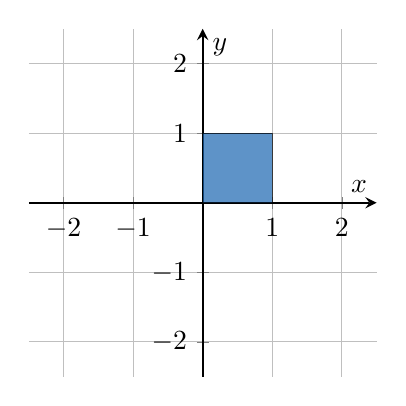
\begin{tikzpicture}
              \begin{axis}[axis x line=center,axis line style = thick,axis y
                line=center,axis
                equal,xmin=-2.5,ymin=-2.5,xmax=2.5,ymax=2.5,xtick={-2,-1,...,2},ytick={-2,-1,...,2},grid=both,xlabel={$x$},ylabel={$y$},width=6cm,height=6cm]
              \addplot[fill=blue,opacity=0.7] coordinates {(0,0) (1,0) (1,1) (0,1)};
              \end{axis}
            \end{tikzpicture}
          \end{center}
        \end{minipage}
        \hspace{2cm}
        \begin{minipage}{.3\textwidth}
          \begin{tikz}
            \draw[-latex,line width=2pt] (1,0) to[out=25,in=155] node[above]{$T$} (2,0);
          \end{tikz}
          
          \vspace{2cm}
        \end{minipage}
        \hspace{-4.5cm}
        \begin{minipage}{.35\textwidth}
          \begin{center}
            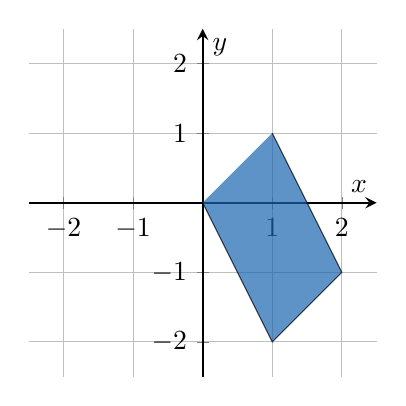
\begin{tikzpicture}
              \begin{axis}[axis x line=center,axis line style = thick,axis y
                line=center,axis
                equal,xmin=-2.5,ymin=-2.5,xmax=2.5,ymax=2.5,xtick={-2,-1,...,2},ytick={-2,-1,...,2},grid=both,xlabel={$x$},ylabel={$y$},width=6cm,height=6cm]
              \addplot[fill=blue,opacity=0.7] coordinates {(0,0) (1,-2) (2, -1) (1,1)};
              \end{axis}
            \end{tikzpicture}
          \end{center}
        \end{minipage}
      \end{center}
      What is the area of $\mathcal{S}$?  What is the area of its image
      $T(\mathcal{S})$?  If $\alpha$ is the standard basis for $\R^2$, what is
      the matrix $[T]_{\alpha \alpha}$ that represents the linear transformation
      $T$?  What is $\mbox{det} [T]_{\alpha \alpha}$?
      
\begin{minipage}{.2\textwidth}
    Area of $\mathcal{S}=$ \makeframednonemptybox{0.5cm}{0.5cm}{1
    }
  \end{minipage}
  \hspace{.2cm}
  \begin{minipage}{.25\textwidth}
    Area of $T(\mathcal{S})=$ \makeframednonemptybox{0.5cm}{0.5cm}{3
    }
  \end{minipage}
  \hspace{.2cm}
  \begin{minipage}{.25\textwidth}
    %% TO ADD YOUR SOLUTION TO THE RECTANGLE, ADD THE NEXT LINE BEFORE EACH ';'
    %% node[midway,blue]{YOUR ANSWER}
    %% 
  $[T]_{\alpha \alpha} = \left[\begin{array}{cc}
            \tikz\draw[black] (0,0) rectangle (5ex,5ex) node[midway,blue]{1};& \tikz\draw[black] (0,0) rectangle (5ex,5ex) node[midway,blue]{1}; \\
            \tikz\draw[black] (0,0) rectangle (5ex,5ex) node[midway,blue]{1};& \tikz\draw[black] (0,0) rectangle (5ex,5ex) node[midway,blue]{-2}; \\
          \end{array}\right]$
   \end{minipage}
   \hspace{.8cm}
   \begin{minipage}{.2\textwidth}
     $\mbox{det} [T]_{\alpha \alpha}=$\makeframednonemptybox{0.5cm}{0.5cm}{-3
    }
   \end{minipage}
      
      \part Consider the linear transformation $T: \R^2 \to \R^2$ given by
      $T((x,y)) = (-x-y,-x/2-y/2)$.  In the domain, draw the unit square
      $\mathcal{S} = \{ (x,y) \mid 0 \leq x \leq 1, 0 \leq y \leq 1 \}$.  In the
      codomain draw the image of the unit square $T(\mathcal{S})$.
      
      \begin{center}
        
        \begin{minipage}{.15\textwidth}
          \begin{center}
            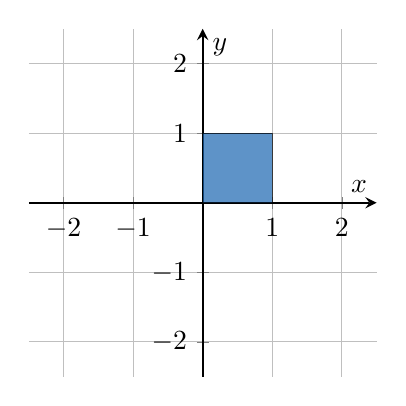
\begin{tikzpicture}
              \begin{axis}[axis x line=center,axis line style = thick,axis y
                line=center,axis
                equal,xmin=-2.5,ymin=-2.5,xmax=2.5,ymax=2.5,xtick={-2,-1,...,2},ytick={-2,-1,...,2},grid=both,xlabel={$x$},ylabel={$y$},width=6cm,height=6cm]
              \addplot[fill=blue,opacity=0.7] coordinates {(0,0) (1,0) (1,1) (0,1)};
              \end{axis}
            \end{tikzpicture}
          \end{center}
        \end{minipage}
        \hspace{2cm}
        \begin{minipage}{.3\textwidth}
          \begin{tikz}
            \draw[-latex,line width=2pt] (1,0) to[out=25,in=155] node[above]{$T$} (2,0);
          \end{tikz}
          
          \vspace{2cm}
        \end{minipage}
        \hspace{-4.5cm}
        \begin{minipage}{.35\textwidth}
          \begin{center}
            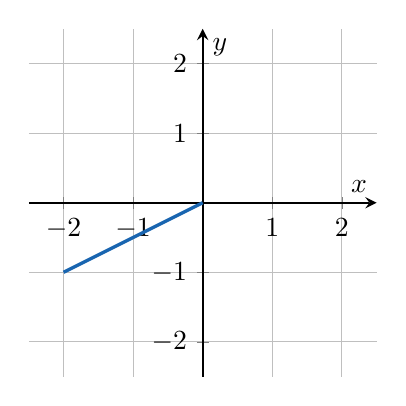
\begin{tikzpicture}
              \begin{axis}[axis x line=center,axis line style = thick,axis y
                line=center,axis
                equal,xmin=-2.5,ymin=-2.5,xmax=2.5,ymax=2.5,xtick={-2,-1,...,2},ytick={-2,-1,...,2},grid=both,xlabel={$x$},ylabel={$y$},width=6cm,height=6cm]
                %\addplot [mark=none,very thick, blue, domain=-2.5:2.5] {1.5*x}; %% USE THIS TO ADD A LINE
                \addplot [mark=none,very thick, blue, domain=-2:0] {0.5*x};
              \end{axis}
            \end{tikzpicture}
          \end{center}
        \end{minipage}
      \end{center}
      What is the area of $\mathcal{S}$?  What is the area of its image
      $T(\mathcal{S})$?  If $\alpha$ is the standard basis for $\R^2$, what is
      the matrix $[T]_{\alpha \alpha}$ that represents the linear transformation
      $T$?  What is $\mbox{det} [T]_{\alpha \alpha}$?

\begin{minipage}{.2\textwidth}
    Area of $\mathcal{S}=$ \makeframednonemptybox{0.5cm}{0.5cm}{1
    }
  \end{minipage}
  \hspace{.2cm}
  \begin{minipage}{.25\textwidth}
    Area of $T(\mathcal{S})=$ \makeframednonemptybox{0.5cm}{0.5cm}{0
    }
  \end{minipage}
  \hspace{.2cm}
  \begin{minipage}{.25\textwidth}
    %% TO ADD YOUR SOLUTION TO THE RECTANGLE, ADD THE NEXT LINE BEFORE EACH ';'
    %% node[midway,blue]{YOUR ANSWER}
    %% 
  $[T]_{\alpha \alpha} = \left[\begin{array}{cc}
            \tikz\draw[black] (0,0) rectangle (5ex,5ex) node[midway,blue]{-1};& \tikz\draw[black] (0,0) rectangle (5ex,5ex) node[midway,blue]{-1}; \\
            \tikz\draw[black] (0,0) rectangle (5ex,5ex) node[midway,blue]{$-\frac{1}{2}$};& \tikz\draw[black] (0,0) rectangle (5ex,5ex) node[midway,blue]{-$\frac{1}{2}$}; \\
          \end{array}\right]$
   \end{minipage}
   \hspace{.8cm}
   \begin{minipage}{.2\textwidth}
     $\mbox{det} [T]_{\alpha \alpha}=$\makeframednonemptybox{0.5cm}{0.5cm}{0
    }
   \end{minipage}
      
      \newpage
      
\part Continuing with the unit square $\mathcal{S}$, as shown in parts (a)--(f), the area of $T(\mathcal{S})$ and
$\mbox{det} [T]_{\alpha \alpha}$ are related. What is the relationship you observed?  Prove this relationship holds for a general linear transformation $T$.  \textit{See question 2(c) for what we mean by a general linear transformation.  Your answer should not need to refer to the entries of $T$; there should be no $a_{12}$ or the like in your answer.} \label{part:area-det}
            
      
      %%% Do not change the height of this box. Your work must fit inside it.
      \makenonemptybox{14cm}{
        %%% Add your explanations here!      
        Area of $T(\mathcal{S}) = \text{Area of }\mathcal{S} \times \mbox{det} [T]_{\alpha \alpha} = \mbox{det} [T]_{\alpha \alpha}$
        Let $V$ be a 2-dimensional vector space and $T: V \to V$ be a general linear transformation for standard basis $\alpha$. We have $\alpha = \{\alpha_1, \alpha_2\} = \{(1,0), (0,1)\}$ hence $\alpha_1$ and $\alpha_2$ encloses the unit square $\mathcal{S}$. Let $v_1, v_2$ be the images of $\alpha_1, \alpha_2$ under $T$ respectively. Then $v_1, v_2$ encloses the image of the unit square $T(\mathcal{S})$ which is a parallelogram. Let $\theta$ be the angle between $v_1$ and $v_2$, we have:
        $$
        P = \text{Area of parallelogram $T(\mathcal{S})$} = |v_1||v_2|\sin\theta
        $$
        Hence, we have:
        $$
        P = |v_1||v_2|\sqrt{1 - \left(\frac{v_1 \cdot v_2}{|v_1||v_2|}\right)^2} = \sqrt{|v_1|^2|v_2|^2 - (v_1 \cdot v_2)^2}
        $$
        Expanding, we have:
        $$
        P = \sqrt{(v_{11}v_{21})^2 + (v_{12}v_{22})^2 + (v_{11}v_{22})^2 + (v_{12}v_{21})^2 - (v_{11}v_{21} + v_{12}v_{22})^2} 
        $$ 
        $$
        = \sqrt{v_{11}^2v_{22}^2 + v_{12}^2v_{21}^2 - 2v_{11}v_{21}v_{12}v_{22}}
        $$
        Simplifying, we have:
        $$
        P = \sqrt{(v_{11}v_{21})^2 + (v_{12}v_{22})^2 - 2v_{11}v_{21}v_{12}v_{22}} = \sqrt{(v_{11}v_{22} - v_{12}v_{21})^2} = |v_{11}v_{22} - v_{12}v_{21}|
        $$
        Let $V = \begin{bmatrix} v_1^\T & v_2^\T \end{bmatrix}$ and $\mathcal{A} = \begin{bmatrix} \alpha_1^\T & \alpha_2^\T \end{bmatrix}$, then $V = \mathcal{A}T$. We have:
        $$
        P = |v_{11}v_{22} - v_{12}v_{21}| = |\text{det}(V)| = |\text{det}(\mathcal{A}T) = |\text{det}(\mathcal{A})\text{det}(T)|.
        $$
        Since $A = \begin{bmatrix} 1 & 0 \\ 0 & 1 \end{bmatrix} = I$, we have $\text{det}(\mathcal{A}) = 1$. Therefore, we have:
        $$
        P = \text{det}(T) = \text{det}[T]_{\alpha \alpha}
        $$
        Hence, the area of $T(\mathcal{S})$ is equal to $|\text{det}[T]_{\alpha \alpha}|$.

        %%% end of your answer    
      }
      
      
      \part If you started with a square of area 4,
      $\mathcal{S}_1 = \{ (x,y) \mid 0 \leq x \leq 2, 0 \leq y \leq 2 \}$ how
      would you use the determinant to compute the area of $T(\mathcal{S}_1)$
      for a general linear transformation?
      
      %%% Do not change the height of this box. Your work must fit inside it.
      \makenonemptybox{4cm}{
        I would use the determinant to compute the area of $T(\mathcal{S}_1)$ for a general linear transformation by:
        $$\text{Area of }T(\mathcal{S}_1) = \text{Area of }\mathcal{S}_1 \times \mbox{det} [T]_{\alpha \alpha} = 4\mbox{det} [T]_{\alpha \alpha}$$
        For all parallelogram $\mathcal{S}_r$ enclosed by two vectors in $V$ with area $A_r$, we can find a linear transformation $Q_r: V \to V$ such that $Q_r(\mathcal{S}_0) = \mathcal{S}_r$ where $\mathcal{S}_0$ is the unit square. Therefore, the area of $\mathcal{S}_r$ is $A_r = \mbox{det} [Q]_{\alpha \alpha}$. Hence $T(\mathcal{S}_r) = T(Q(\mathcal{S}_0))$. From part \ref{part:area-det}, we have $T(\mathcal{S}_r) = T(Q(\mathcal{S}_0)) = \mbox{det} [TQ]_{\alpha \alpha} = \mbox{det} [T]_{\alpha \alpha}\mbox{det} [Q]_{\alpha \alpha} = A_r\mbox{det} [T]_{\alpha \alpha}$. Also, since $Q_r(\mathcal{S}_0) = \mathcal{S}_r$ from part \ref{part:area-det}, we have $\mbox{det} [Q]_{\alpha \alpha} = A_r$. Therefore, the area of $T(\mathcal{S}_r)$ is $A_r\mbox{det} [T]_{\alpha \alpha}$.\\
        In this case where $\mathcal{S}_1$ is a square of area 4, the area of $T(\mathcal{S}_1)$ is $4\mbox{det} [T]_{\alpha \alpha}$.

      }
      
      
    \end{parts}
    
    \newpage
    
    \begin{EnvUplevel}
      
      \textbf{The following question 4 is worth zero points.  Your work will not be
        graded.  The question generalizes the previous question and is within your
        reach if you are comfortable with dot products and cross products.  It is
        material that you may be assumed to already know when you're in AER210.  We
        encourage you to think about and work on this problem and we are happy to
        talk about it with you, but it is provided ``for the curious'' in that you
        will not be tested on it.}
      
      \textbf{YOU MUST UPLOAD THIS PAGE EVEN IF YOU WROTE NOTHING ON IT.}
      
    \end{EnvUplevel}
    
    \question What about volumes of parallelepipeds?
    
    \begin{minipage}{.6\textwidth}
      Each face of a parallellepiped is parallel to the opposite face; the
      parallelepiped is determined by the three edges coming out from any one
      corner.  In the image, we have a corner at $(0,0,0)$ and the three edges are
      represented using the vectors in $\ba, \bb, \bc \in {^3}\R$, for example the
      vectors based at the origin $(0,0,0)$.
    \end{minipage}
    \begin{minipage}{.35\textwidth}
      \flushright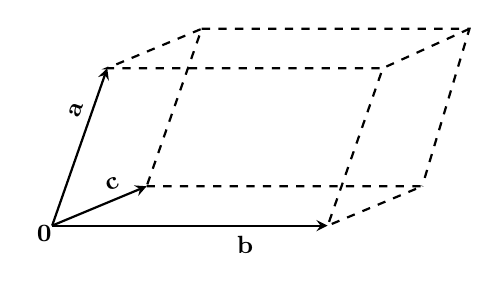
\begin{tikzpicture}
        \draw[-stealth,thick] (0,0) -- (0.7,2) node[pos=0.7,above,rotate=70.7] {\small$\textbf{a}$};
        \draw[-stealth,thick] (0,0) -- (3.5,0) node[pos=0.7,below] {\small$\textbf{b}$};
        \draw[-stealth,thick] (0,0) -- (1.2,0.5) node[pos=0.7,above,rotate=22.6] {\small$\textbf{c}$};
        \draw[dashed,thick] (1.2,0.5) -- (4.7,0.5) -- (3.5,0) -- (4.2,2) -- (0.7,2) -- (1.9,2.5) -- (1.2,0.5);
        \draw[dashed,thick] (1.9,2.5) -- (5.3,2.5) -- (4.7,0.5);
        \draw[dashed,thick] (5.3,2.5) -- (4.2,2);
        \node at (-0.1,-0.1) {\small$\mathbf{0}$};
      \end{tikzpicture}
    \end{minipage}
    
    
    To find the volume of a parallelepiped\footnote{A parallelepiped is a solid
      object with corners and edges and an interior.  We can understand it using
      Cartesian coordinates the moment we say where the origin is and where the
      $x$, $y$, and $z$ axes are.  In the picture we're implicitly taking the
      view that the positive $x$ axis is in the same direction as $\bb$, the
      positive $y$ axis is in the same direction as $\bc$, and the positive $z$
      axis is in the same direction as $\ba$.  But we need to be careful to
      remember that edges are collections of points like $(0,0,0)$ and $(1,0,0)$
      and so forth while the vectors $\ba$, $\bb$, and $\bc$ are in $^3\R$.},
    you need to find the area of one face and the distance of the opposite face
    to that one face.  For example, if you found the area of the bottom face
    (the one determined by $\bb$ and $\bc$) you would need to find the height of
    the parallelepiped.  You would then multiply the two areas.
    
    \begin{parts}
      \part Using the above figure, explain why the volume of the parallelipiped
      is $| \ \ba \cdot ( \bb \times \bc ) \ |$.  Explain how this is related to
      the determinant of the matrix whose rows are given by $\ba$, $\bb$, and
      $\bc$:
      $$
      \det \begin{bmatrix} \ba^\T \\ \bb^\T \\ \bc^\T \end{bmatrix}.
      $$
      
      %%% Do not change the height of this box. Your work must fit inside it.
      \makenonemptybox{8cm}{
        %%% Add your explanations here!      
        
        %%% end of your answer    
      }
      
      \newpage
      
          \begin{EnvUplevel}
      
      \textbf{YOU MUST UPLOAD THIS PAGE EVEN IF YOU WROTE NOTHING ON IT.}
      
    \end{EnvUplevel}
    
      
      \part Explain why you would have gotten the same volume if you had based your
      calculation on the front of the parallelepiped (determined by $\ba$ and $\bb$)
      or if you had based your calculation on the side of the parallelepiped
      (determined by $\ba$ and $\bc$).
      $$
      \mbox{volume of parallelepiped} = \det \begin{bmatrix} \bc^\T \\ \ba^\T \\
        \bb^\T \end{bmatrix} = \det \begin{bmatrix} \bb^\T \\ \bc^\T \\
        \ba^\T \end{bmatrix}.
      $$
      
      %%% Do not change the height of this box. Your work must fit inside it.
      \makenonemptybox{18cm}{
        %%% Add your explanations here!      
        
        %%% end of your answer    
      }
      
      \newpage
      
                \begin{EnvUplevel}
      
      \textbf{YOU MUST UPLOAD THIS PAGE EVEN IF YOU WROTE NOTHING ON IT.}
      
    \end{EnvUplevel}
    
      
      \part Consider the unit cube
      $\mathcal{C} = \{ (x,y,z) \mid 0 \leq x \leq 1, 0 \leq y \leq 1, 0 \leq z \leq
      1\}$.  Let $T: \R^3 \to \R^3$ be a linear transformation.  What is the image
      of $\mathcal{C}$?  (What is $T(\mathcal{C})$ geometrically?)  If $\alpha$ is
      the standard basis for $\R^3$ and $[T]_{\alpha \alpha}$ is the matrix that
      represents the linear transformation, what is $\det [T]_{\alpha \alpha}$ and
      how does it relate to the volume of $T(\mathcal{C})$?
      
      %%% Do not change the height of this box. Your work must fit inside it.
      \makenonemptybox{14cm}{
        %%% Add your explanations here!      
        
        %%% end of your answer    
      }
      
      
      
      \part If you started with a cube of volume 8,
      $\mathcal{C}_1 = \{ (x,y,z) \mid 0 \leq x \leq 2, 0 \leq y \leq 2, 0 \leq z
      \leq 2\}$, how would you use the determinant to compute the volume of
      $T(\mathcal{C}_1)$?
      
      %%% Do not change the height of this box. Your work must fit inside it.
      \makenonemptybox{3.0cm}{
        %%% Add your explanations here!      
        
        %%% end of your answer    
      }
      
      
    \end{parts}
    
    
    
    
  \end{questions}
  
\end{document}
